\section{Program Oversigt}
Denne sektion omhandler strukturen af programmet med udgangspunkt fra 'GUIMain', programmets start og hoved vindue. 

\begin{figure}[!h]
    \centering
    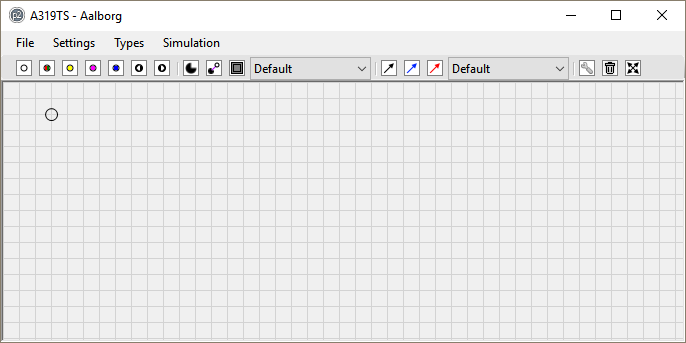
\includegraphics[width=\textwidth,height=\textheight,keepaspectratio]{Pictures/Implementation/program}
    \caption{Programmets hoved vindue 'GUIMain'}
    \label{a319program}
\end{figure}

På figur \ref{a319program} ses GUIMain. GUIMain består af en menulinje, værktøjslinje og en viewport. Vinduet fungerer udelukkende ved brug af events. Ved tryk på et menupunkt, vil der udløses en event, der åbner det tilsvarende vindue. Menupunkterne er delt op i 4 forskellige kategorier. File indeholder menupunkter der håndtrer fil åbning og gemning. Settings har indstillinger til det nuværende projekt, fordeling af destinationer og transportmiddelvalg, og sidst indstillinger for hvordan simuleringen skal udføres. Types har menupunkter til opsætning af forskellige destination, vej og køretøj typer. Sidst kan man igennem 'Simulation' køre og vise simuleringer.

\vspace{5mm}

Værktøjslinjen har en række knapper der kan tjekkes. Når en knap bliver trykket på, bliver der sendt en event der kalder metoden 'ToggleTool' på ToolControlleren. ToggleTool sørger for at der kun er en aktiv knap ad gangen. Derudover er der to lister på værktøjslinjen, i listen til venstre kan brugeren vælge destinations typen der bliver brugt, og i listen til højre kan brugeren vælge hvilken vejtype der skal bruges.

\vspace{5mm}

Viewporten er gitteret hvor der er muligt at opstille et vejnet. Viewporten abonnerer på 'Move' og 'Click' begivenhederne. Hver gang brugeren flytter musen, vil viewporten finde ud af hvor musen er, og tegne en cirkel, så brugeren kan være sikker på, hvilken gitter position der vil blive tilføjet til på forhånd. Ved tilfældet at brugeren trykket på viewporten, tjekker ToolControlleren efter hvilket værktøj der er aktivt, og kører metoden der er forbundet til værktøjet.